\documentclass[hyphens]{beamer}

\usepackage[utf8]{inputenc}
\usepackage[ngerman]{babel}

\usepackage{array}
\usepackage{tabularx}
\newcolumntype{Z}{>{\raggedright\let\newline\\\arraybackslash}X}

\usepackage{amssymb}
\usepackage{pifont}
\newcommand{\xmark}{\ding{55}}
\usepackage{svg}
\usepackage[autostyle]{csquotes}
\usepackage{minted}
\usepackage{tikz}
\usetikzlibrary{mindmap,trees}

\usetheme{Execushares}

\setbeamertemplate{section in toc}[sections numbered]
\setbeamertemplate{subsection in toc}{\leavevmode\leftskip=2em%
	\inserttocsectionnumber.\inserttocsubsectionnumber~%
	\inserttocsubsection\par}
\setbeamertemplate{caption}{\raggedright\insertcaption\par}

\begin{document}
  \title[Gerät zur Schlaganfall-Rehabilitation]{\LARGE{Entwicklung eines Gamification-basierten Unterstützungs- und Motivationsgeräts zur Rehabilitation von Schlaganfall-Patienten}}
  \subtitle{Kolloquium am Spezialschulteil des staatlichen Gymnasiums "'Albert Schweitzer"' Erfurt}
  \author[Lukas Rost]{Lukas Rost \\ \emph{Fachbetreuer:} Johannes Süpke \\ \emph{Außenbetreuer:} Hannes Weichel}
  \date{20. März 2019}


 \titlepage
 
 \begin{frame}
 \begin{figure}
 	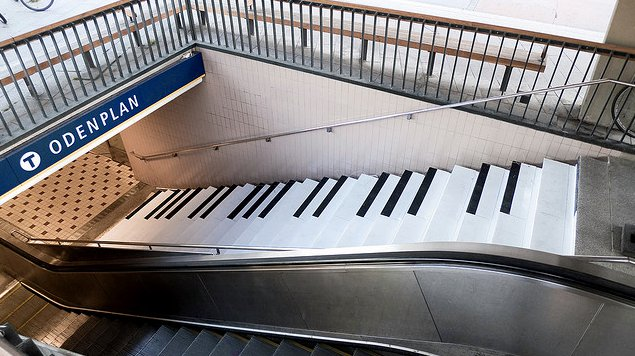
\includegraphics[scale=0.5]{pics/pianostairs}
 	\caption{\href{https://www.youtube.com/watch?v=SByymar3bds}{Die Klaviertreppe aus dem Projekt \textsc{The Fun Theory}}}
 \end{figure}
\end{frame}

 
 \titlepage

 \begin{frame}{Gliederung}
 \tableofcontents
 \end{frame}

\section{Schlaganfall und Therapiemethoden}

\begin{frame}{Schlaganfall als Krankheitsbild}
\begin{figure}
	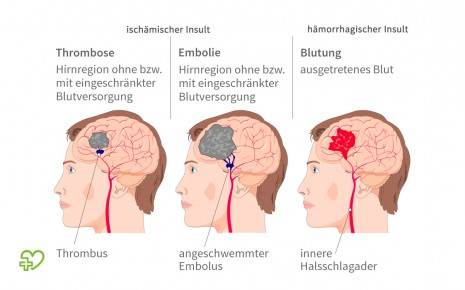
\includegraphics[scale=0.6]{pics/sentst}
	\caption{Arten des Schlaganfalls}
\end{figure}
\end{frame}

\begin{frame}{Schlaganfall als Krankheitsbild}
\begin{figure}
	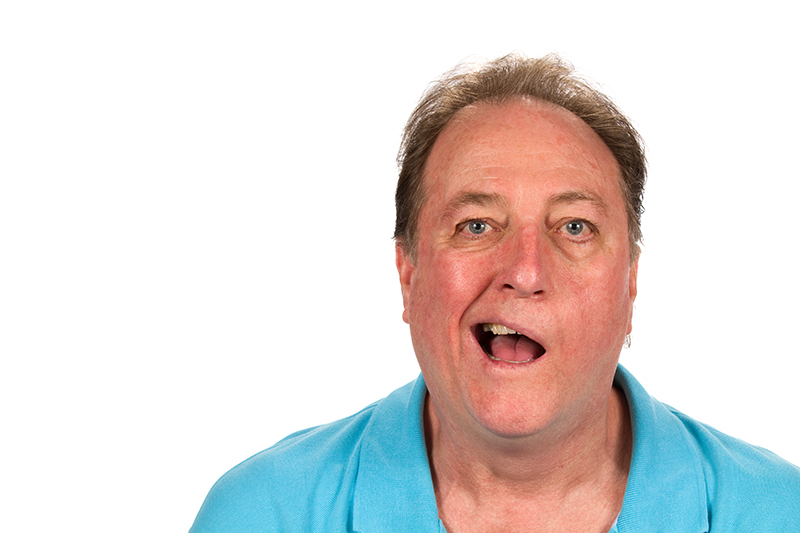
\includegraphics[scale=1.1]{pics/laehm}
	\caption{Gesichtslähmung als Symptom eines Schlaganfalls}
\end{figure}
\end{frame}

\begin{frame}{Schlaganfall als Krankheitsbild}
\begin{figure}
	\includesvg[scale=1.2]{pics/Schlaganfall}
	\caption{Schaubild zum FAST-Test}
\end{figure}
\end{frame}

\begin{frame}{Mögliche Therapiemethoden}
	\begin{itemize}
		\item Constraint-Induced Movement Therapy
		\item Bobath-Konzept
		\item bilaterales Training
		\item schädigungsorientiertes Training
		\begin{itemize}
			\item Arm-Basis-Training
			\item Arm-Fähigkeits-Training
		\end{itemize}
		\item aufgabenorientiertes Training
		\item technische Ansätze
		\begin{itemize}
			\item Armrobot
			\item Elektrostimulation
		\end{itemize}
	\end{itemize}
\end{frame}

\begin{frame}{Mögliche Therapiemethoden}
\begin{figure}
	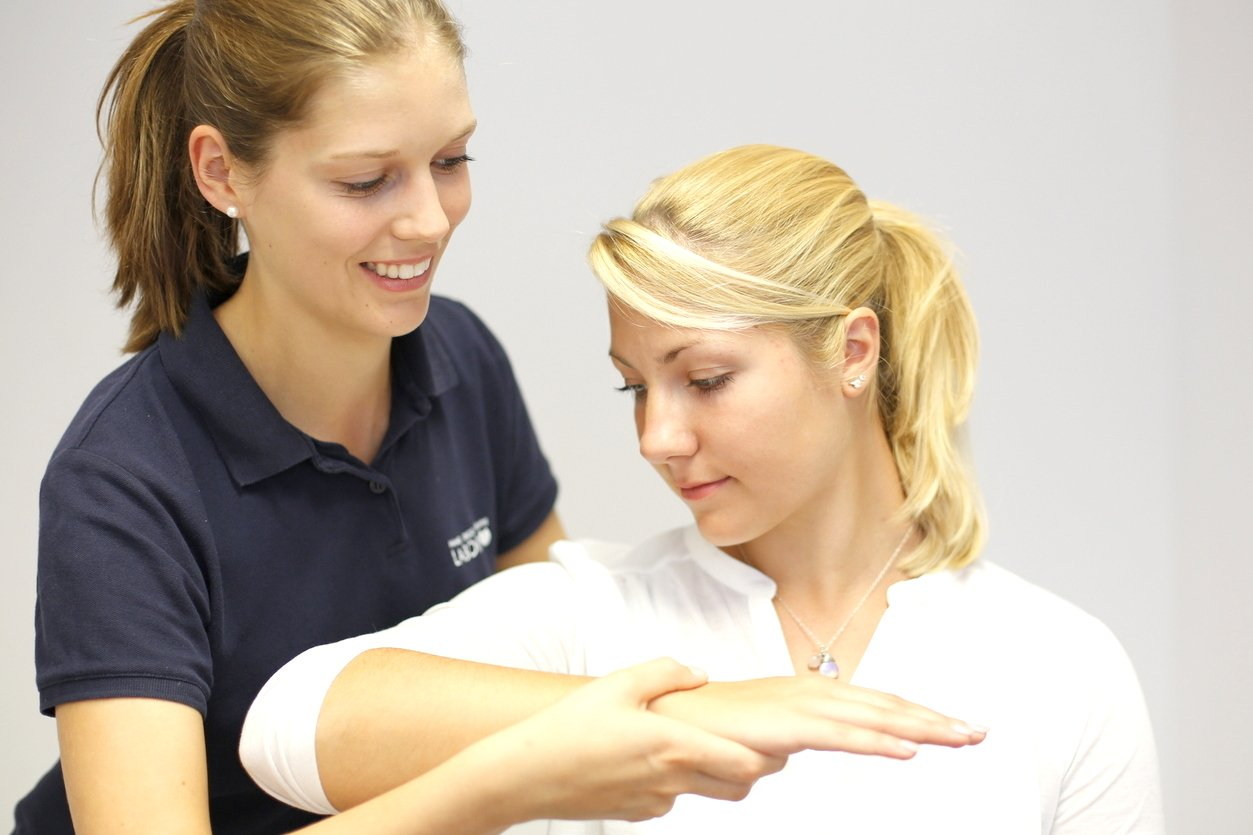
\includegraphics[scale=0.2]{pics/armbasis}
	\caption{Übung während des Arm-Basis-Trainings}
\end{figure}
\end{frame}

\begin{frame}{Mögliche Therapiemethoden}
\begin{figure}
	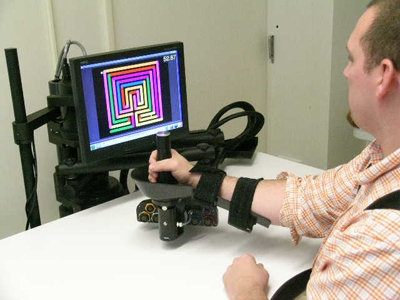
\includegraphics[scale=0.6]{pics/armrobot}
	\caption{Ein Armrobot-Gerät}
\end{figure}
\end{frame}

\section{Motivation durch Gamification}

\subsection{Mechanismen und Merkmale}

\begin{frame}{Mechanismen und Merkmale}
\textbf{Definition:} \\
\blockquote{Verwendung von spieltypischen Mechaniken außerhalb reiner Spiele, mit dem Ziel, das Verhalten von Menschen zu beeinflussen}
\hspace{0.5cm}
\begin{itemize}
	\item \textbf{Ziel:} Steigerung der Nutzungsmotivation
	\item Ausnutzung des menschlichen Spieltriebs
	\item Resultatstransparenz
	\item operante Konditionierung
\end{itemize}
\end{frame}

\begin{frame}{Mechanismen und Merkmale}
\begin{figure}
	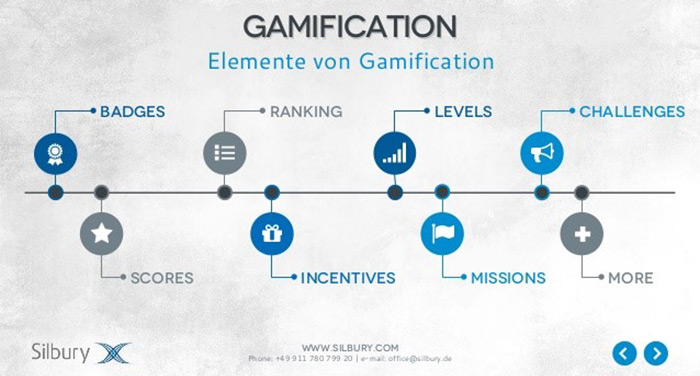
\includegraphics[scale=0.45]{pics/elements}
	\caption{Spieltypische Mechanismen und Elemente}
\end{figure}
\end{frame}

\subsection{Beispiele für die motivationssteigernde Wirkung}

\begin{frame}{Motivationssteigernde Wirkung}
\begin{figure}
	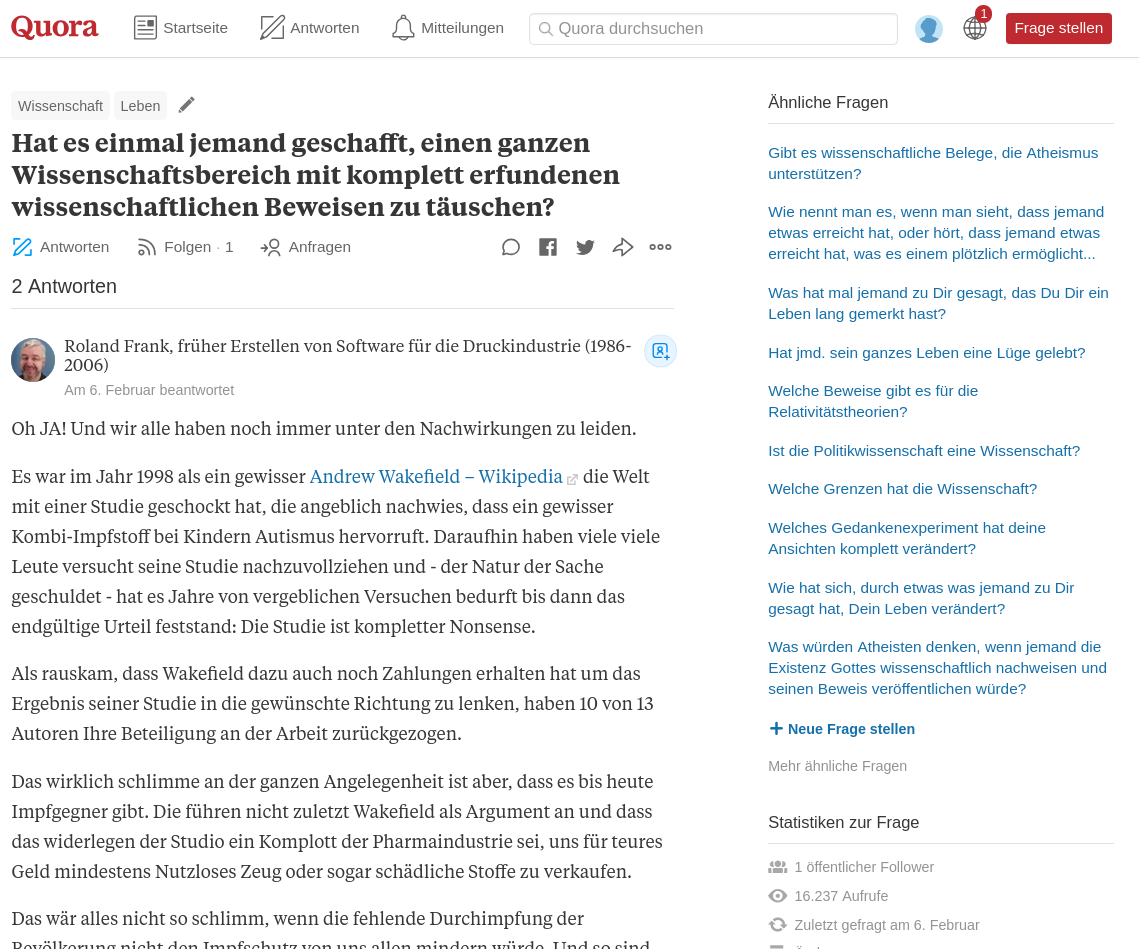
\includegraphics[scale=0.16]{pics/quora}
	\caption{Die Frage-Antwort-Website Quora}
\end{figure}
\end{frame}

\section{Schaltung und Implementierung des Geräts}

\subsection{Aufbau der Schaltung}

\begin{frame}{Aufbau der Schaltung}
	\begin{itemize}
		\item Elektromyografie-Sensor
		\item Mikrocontroller Atmel ATmega 88PA
		\item Bluetooth-Chip HC-05
		\item Quarzoszillator und Kondensatoren
	\end{itemize}
\end{frame}

\begin{frame}{Aufbau der Schaltung}
\begin{figure}
	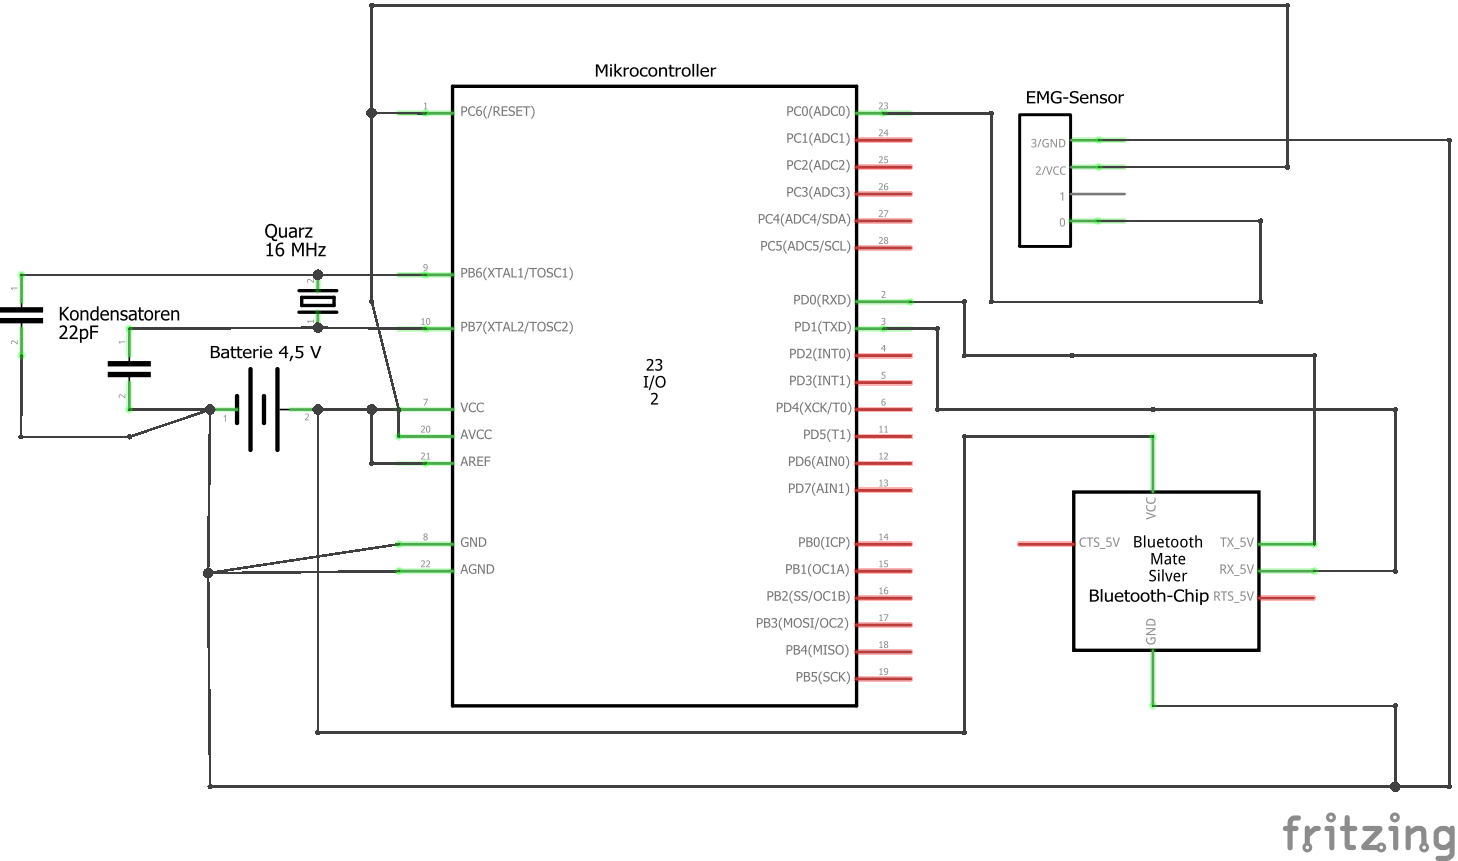
\includegraphics[scale=0.7]{pics/mikrocontroller-schaltplan}
	\caption{Der Schaltplan des Geräts}
\end{figure}
\end{frame}

  \begin{frame}{Aufbau der Schaltung}
\begin{figure}
	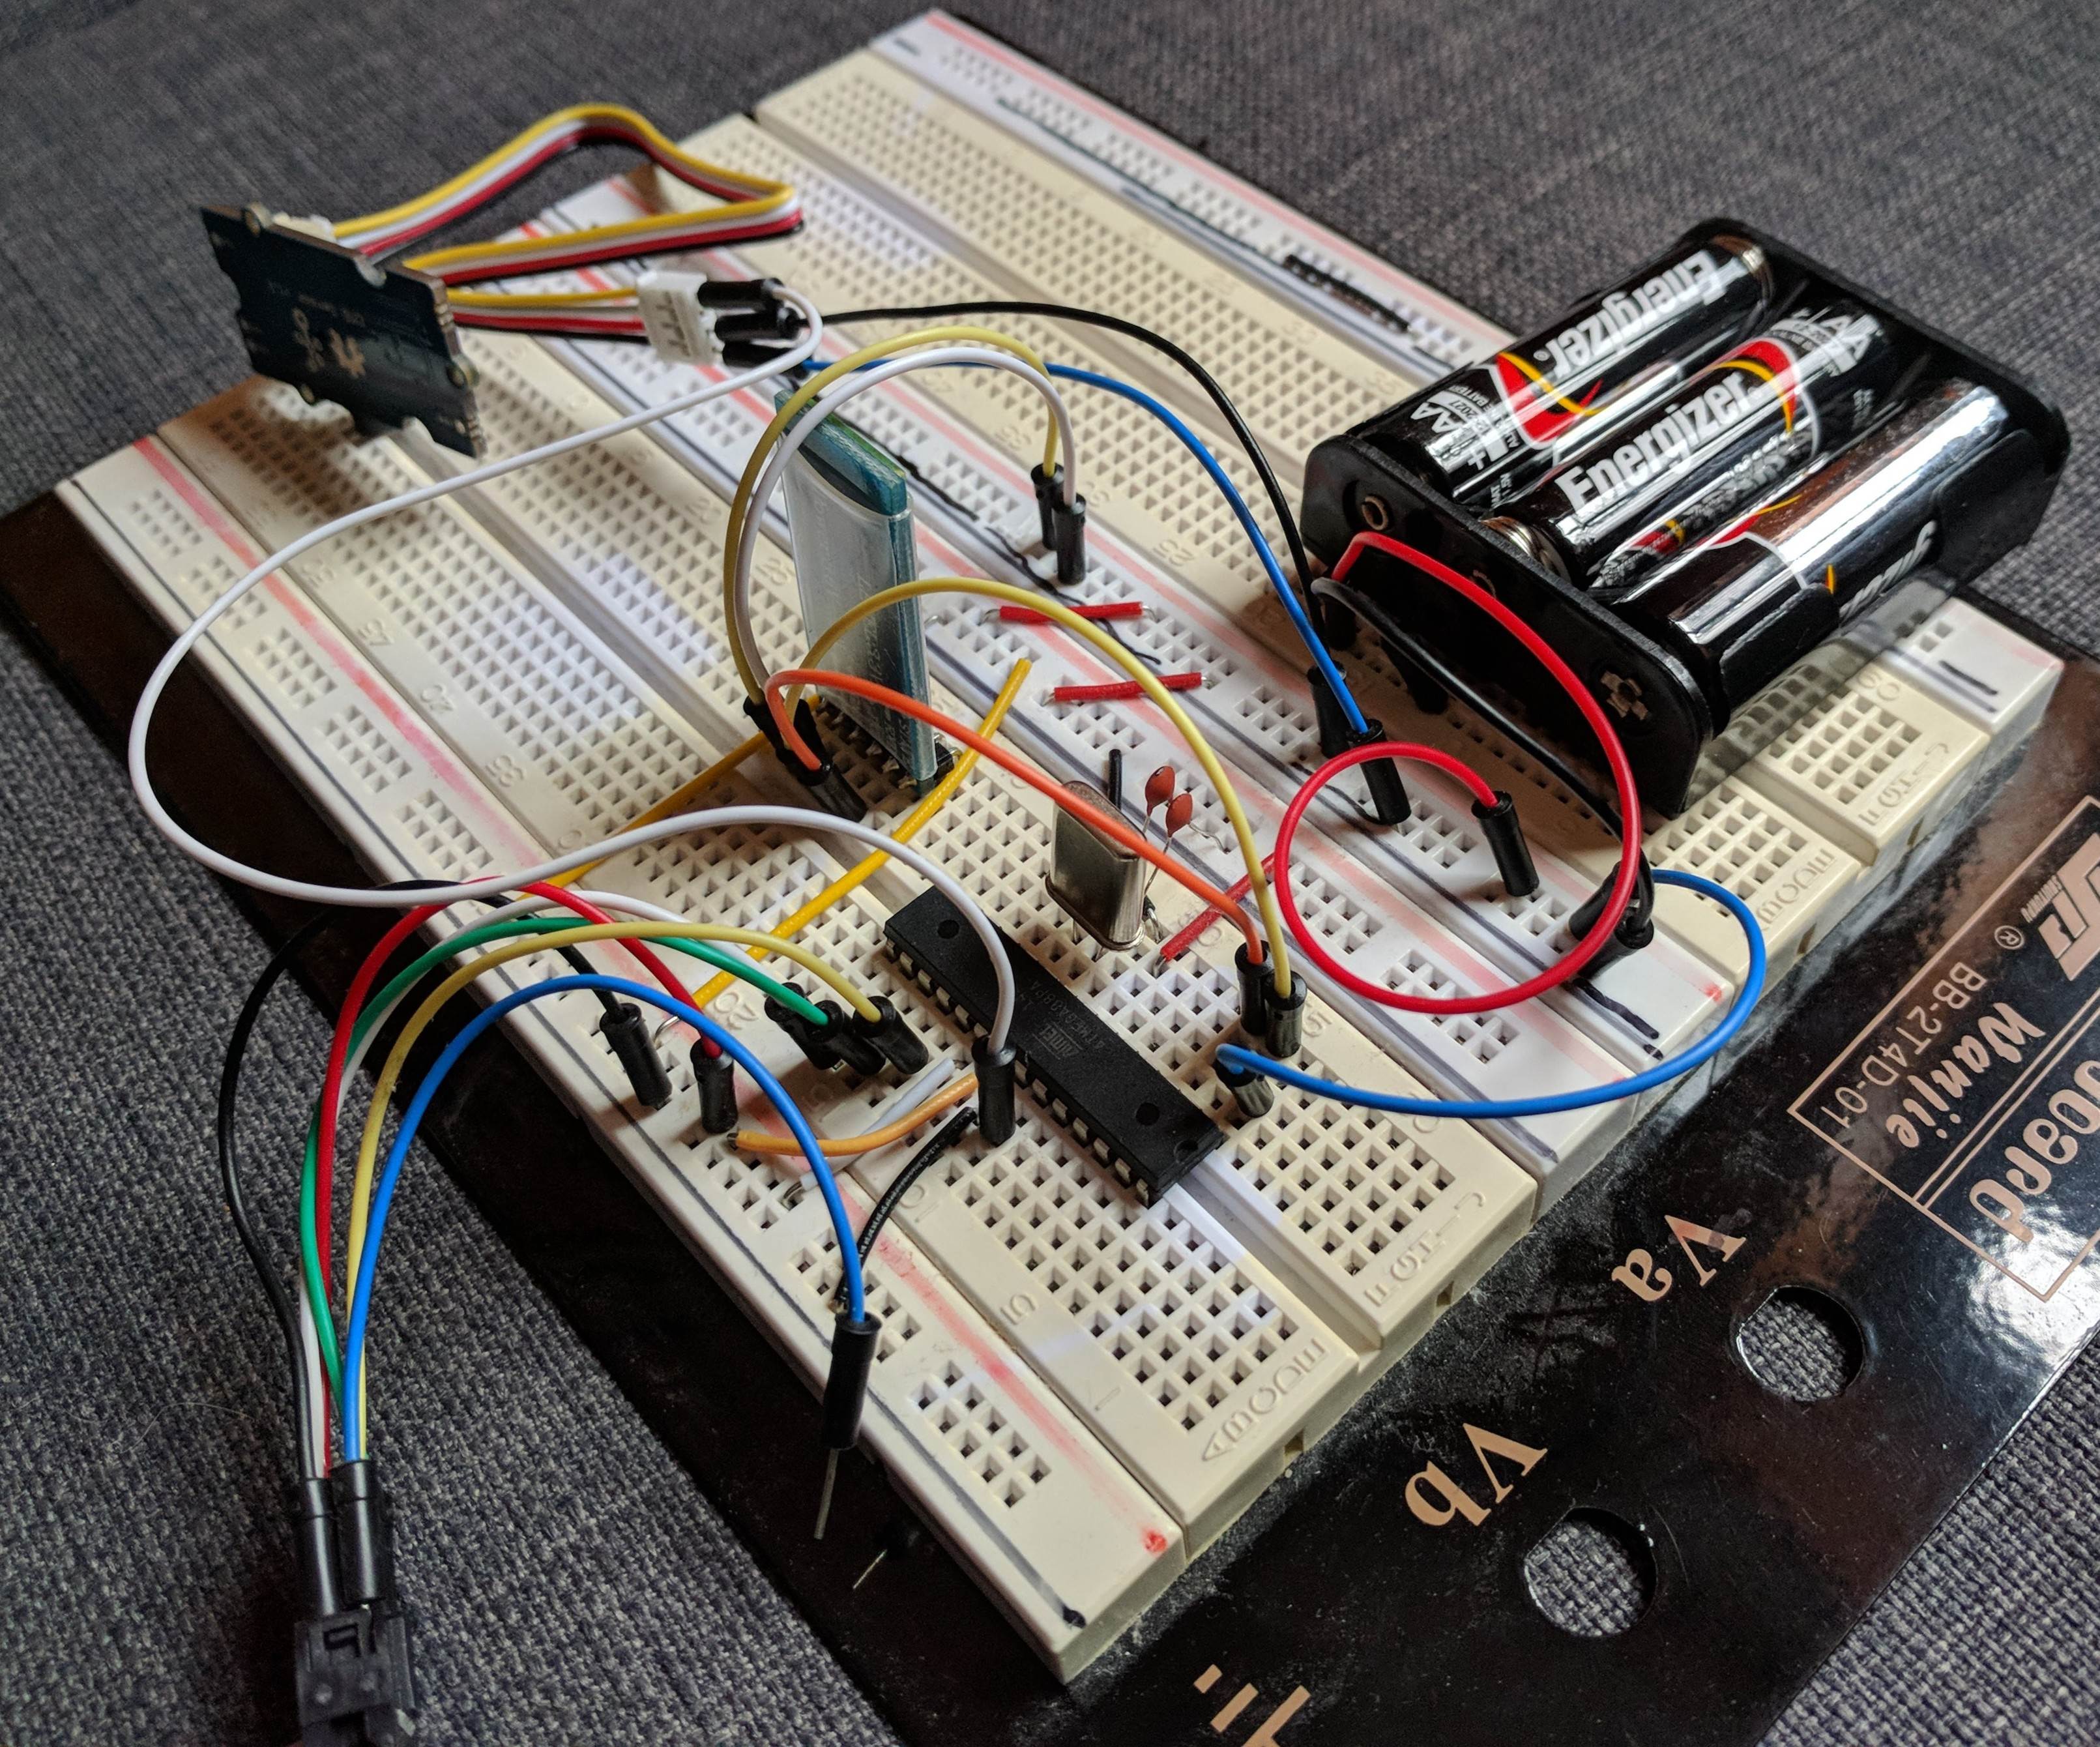
\includegraphics[scale=0.06]{pics/mikro}
	\caption{aufgebaute Schaltung auf einem Breadboard}
\end{figure}
\end{frame}

\subsection{Implementierung des Programms}

\begin{frame}[fragile]{Implementierung des Programms}
	\begin{figure}
	\begin{minted}[frame=single]{c}
void sendCurrentVoltage(void) {
	ADCSRA |= (1 << ADSC);
	while (ADCSRA & (1 << ADSC));
	uint16_t out = ADC;
	double voltage = (out/1024.0) * 4.5;
	
	char str[10];
	sprintf(str, "%.3f \r\n", voltage);
	u_puts(str);
}
	\end{minted}
	\centering \caption{Ausschnitt aus dem Programm}
\end{figure}
\end{frame}

\section{Entwicklung der Begleitapp}

\subsection{Konzept und Aufbau der App}

\begin{frame}[fragile]{Konzept und Aufbau der App}
\tikzset{level 1 concept/.append style={font=\sf, sibling angle=90,level distance = 32mm}}
\tikzset{level 2 concept/.append style={font=\sf, sibling angle=45,level distance = 27mm}}
\tikzset{every node/.append style={scale=0.7,text width=}}
\begin{center}
	\begin{tikzpicture}
	\path [
	mindmap,
	text = white,
	level 1 concept/.append style =
	{font=\Large\bfseries, sibling angle=100},
	level 2 concept/.append style =
	{font=\normalsize\bfseries},
	level 3 concept/.append style =
	{font=\small\bfseries},
	style = {concept color=black,
		font=\Large\bfseries},
	engines/.style = {concept color=green!50!black},
	formats/.style = {concept color=blue!50!black}
	]
	node [concept] {Begleitapp} [clockwise from=330]
	child[concept color=green!50!black, nodes={engines}] {
		node [concept] {Funktionen} [clockwise from=0]
		child { node [concept] {Übungen} }
		child { node [concept] {Minispiel} }
		child { node [concept] {Gamification} }
		child { node [concept] {Erinnerungen} }}
	child [concept color=blue!50!black, nodes={formats}] {
		node [concept] {Aufbau} [clockwise from=270]
		child { node [concept] {Start} }
		child { node [concept] {Übungen} }
		child { node [concept] {Minispiel} }
		child { node [concept] {Einstellungen} }
	};
	\end{tikzpicture}
\end{center}
\end{frame}

\subsection{Kommunikation mit dem Mikrocontroller}

\begin{frame}{Kommunikation mit dem Controller}
\begin{itemize}
	\item Berechnung eines Prozentsatzes:
	\begin{equation*}
	p = 100 * \frac{x - U_{min}}{U_{max} - U_{min}}
	\end{equation*}
\end{itemize}
\end{frame}

\begin{frame}{Kommunikation mit dem Controller}
	\begin{figure}
		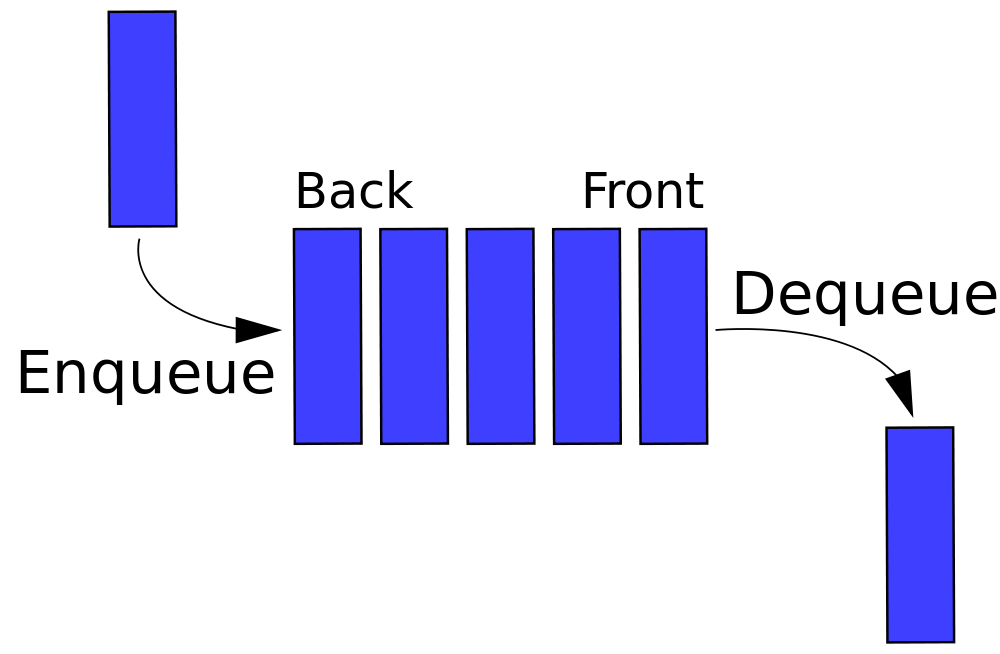
\includegraphics[scale=0.28]{pics/queue}
		\caption{Funktionsweise einer Warteschlange (Queue)}
	\end{figure}
\end{frame}

\subsection{Umsetzung der Gamification}

\begin{frame}{Umsetzung der Gamification}
\begin{figure}
	\includesvg[scale=0.55]{pics/reldb}
	\caption{Eine Tabelle einer relationalen Datenbank}
\end{figure}
\end{frame}

\begin{frame}[fragile]{Umsetzung der Gamification}
\tikzset{level 1 concept/.append style={font=\sf, sibling angle=90,level distance = 32mm}}
\tikzset{level 2 concept/.append style={font=\sf, sibling angle=45,level distance = 30mm}}
\tikzset{every node/.append style={scale=0.65,text width=}}
\begin{center}
	\begin{tikzpicture}
	\path [
	mindmap,
	text = white,
	level 1 concept/.append style =
	{font=\Large\bfseries, sibling angle=140},
	level 2 concept/.append style =
	{font=\normalsize\bfseries},
	level 3 concept/.append style =
	{font=\small\bfseries},
	style = {concept color=black,
		font=\Large\bfseries},
	engines/.style = {concept color=green!50!black},
	formats/.style = {concept color=blue!50!black}
	]
	node [concept] {Quest-Tabelle} [clockwise from=305]
	child[concept color=green!50!black, nodes={engines}] {
		node [concept] {Anzeige} [clockwise from=310]
		child { node [concept] {ID} }
		child { node [concept] {Titel} }
		child { node [concept] {Beschreibung} }
		child { node [concept] {Symbol} }
	}
	child [concept color=blue!50!black, nodes={formats}] {
		node [concept] {Anforderungen} [clockwise from=270]
		child { node [concept] {Anzahl an XP} }
		child { node [concept] {Wert übertreffen} }
		child { node [concept] {Wert übertr. (Dauer)} }
	}
	child[concept color=orange!50!black]{
		node [concept] {Beendet?}
	};
	\end{tikzpicture}
\end{center}
\end{frame}

\begin{frame}{Umsetzung der Gamification}
\textbf{XP-Vergabe:}
\begin{itemize}
	\item Punktzahl $P$ für eine Übung:
	\begin{flalign*}
	& P = \frac{min(L) + avg(L) + max(L)}{3}&
	\end{flalign*}
	\item Punktzahl $P_{S}$ für ein Minispiel:
	\begin{flalign*}
	& P_{S} = P + 2 \cdot d&
	\end{flalign*}
	\item beim Beenden einer Quest
\end{itemize}
\end{frame}

\section*{Demonstration}

 \section*{Kritische Reflexion des Erreichten}
 \begin{frame}{Kritische Reflexion des Erreichten}
 	\begin{table}
 		\begin{tabularx}{\textwidth}{|Z|c|}
 			\hline
 			\textbf{Ziel} & \textbf{Erreicht?} \\
 			\hline
 			\hline
 			Entwicklung eines funktionstüchtigen Prototypen des Geräts & \checkmark \\
 			\hline
 			Konzipierung und Implementierung einer entsprechenden Begleitapp & \checkmark \\
 			\hline
 			Nutzung der zur Verfügung gestellten Seminarfachtage  & \checkmark \\
 			\hline
 			weitestgehende Einhaltung des Zeitplans & \checkmark \\
 			\hline
 			Behebung aller Fehler in der Schaltung & \xmark \\ 
 			\hline
 			Test an realen Schlaganfallpatienten & \xmark \\ 
 			\hline
 			Entwicklung eines serienmäßig produzierbaren Geräts (\emph{kein Ziel!}) & \xmark \\ 
 			\hline
 		\end{tabularx}
 	\end{table}
 \end{frame}

 \begin{frame}{Bildquellen}
 \begin{itemize}
 \item \small{\url{http://www.lahsit-schlaganfall-reha.de/images/slider/lahsit-banner-3.png}}
 \item \small{\url{https://i.onmeda.de/schlaganfall_entstehung-465x290.jpg}}
 \item \small{\url{http://www.volkskrankheiten.at/images/1237/widgets/Schlaganfall-(2).svg}}
 \item  \small{\url{https://www.neurozentrum-bern.ch/wp-content/uploads/2015/01/diagnose_schlaganfall.jpg}}
 \item  \small{\url{http://news.mit.edu/sites/mit.edu.newsoffice/files/styles/news_article_image_top_slideshow/public/images/2010/20100414154658-1_0.jpg}}
 \end{itemize}
 \end{frame}

 \begin{frame}{Bildquellen}
\begin{itemize}
	\item \small{\url{http://www.lahsit-schlaganfall-reha.de/images/Laborn-Armbasistraining.JPG}}
	\item \small{\url{http://blog.brandung.de/wp-content/uploads/2017/03/gmf-01.jpg}}
	\item \small{\url{https://de.quora.com/Hat-es-einmal-jemand-geschafft-einen-ganzen-Wissenschaftsbereich-mit-komplett-erfundenen-wissenschaftlichen-Beweisen-zu-täuschen}}
	\item \small{\url{https://upload.wikimedia.org/wikipedia/commons/1/1b/Begriffe_relationaler_Datenbanken.svg}}
	\item \small{\url{https://scontent-frx5-1.xx.fbcdn.net/v/t1.0-9/225807_10150179024982659_311531_n.jpg?_nc_cat=0&oh=986b13c0619d22e40dc9de883a6ed930&oe=5B5CEE4C}}
\end{itemize}
\end{frame}

 \titlepage

\end{document}
